% Author: Rasmus Pank Roulund

\usetikzlibrary{shapes,arrows,positioning}
\tikzstyle{block} = [draw, fill=white, rectangle, 
    minimum height=2em, minimum width=7em]
\tikzstyle{input} = [coordinate]
\tikzstyle{output} = [coordinate]
\tikzstyle{pinstyle} = [pin edge={to-,thin,black}]
\begin{figure}[htbp]
\centering
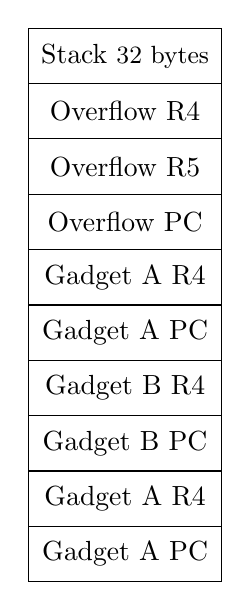
\begin{tikzpicture}[auto, node distance=2em,>=latex']
% \begin{scope}[node distance=3em and 20em]%Here we change it for everything inside this scope
  % \node [block,name=stack] {Stack};
  % \node [output, right= 2em of stack] (rstack) {};
  % \node [output, left= 2em of stack] (lstack) {};


  \node [block] (uname) {Stack {\small32 bytes}};
  \node [block,below of=uname] (passd) {Overflow R4};
  \node [block,below of=passd] (pass1) {Overflow R5};
  \node [block,below of=pass1] (pass2) {Overflow PC};
  \node [block,below of=pass2] (pass3) {Gadget A R4};
  \node [block,below of=pass3] (pass4) {Gadget A PC};
  \node [block,below of=pass4] (pass5) {Gadget B R4};
  \node [block,below of=pass5] (pass6) {Gadget B PC};
  \node [block,below of=pass6] (pass7) {Gadget A R4};
  \node [block,below of=pass7] (pass8) {Gadget A PC};
  % \node [output, right= 2em of uname] (runame) {};
  % \node [output, right= 2em of passd] (rpassd) {};
  % \node [output, right= 2em of pass1] (rpass1) {};
  % \node [output, right= 2em of pass2] (rpass2) {};
 
  % \node [output, left= 2em of uname] (luname) {};
  % \node [output, left= 2em of passd] (lpassd) {};
  % \node [output, left= 2em of pass1] (lpass1) {};
  % \node [output, left= 2em of pass2] (lpass2) {};



  % \draw [->] (uname) -- (runame) -- (rpassd) -- (passd);
  % \draw [->] (stack) -- (lstack) -- (luname) -- (uname);

\end{tikzpicture}
\caption{The stack configuration. }
\label{fig::stack}
\end{figure}
% \begin{lstlisting}
% bottom of 
% memory    

% \end{lstlisting}